\section{Complexity in Languages\timeestimation{30h}}
\label{sec:complexity}
While most languages we encounter are turing-complete, that does not need
to be the case. In this chapter, we will discuss the notion of a problem 
description as a programming language.

\subsubsection{Problem descriptions}
There are many different kinds of problems in computer science, for example 
sorting a list or determining if a boolean formula with variables is always
true. Nevertheless, these kind of problems are never singular -- we would not 
want an algorithm\footnote{Most definitions would not even allow this as an 
algorithm}, that could reliably sort the list $4, 8, 2, -9$, but one that 
could sort \emph{all} lists, no matter the size. This means of course, that 
algorithms need data as input to describe the problems they need to solve. 
This data is then called the \emph{problem description}. 

Looking back at the beginning, the semantic function was introduced to give 
meaning to data. Since then, we primarily used it to differentiate between 
\WHILE programs and the functions they denote. In the case of problem
descriptions, we can the interpretation of a problem would be the solution 
that we would expect. 

\begin{example}
	$U = Cons(Nil, Cons(Nil, Cons(Nil, Nil)))$, then $\interpret[unary]{U} = 3$.
\end{example}
\begin{example}
	$L=Cons(4, Cons(8, Cons(2, Cons(-9, Nil))))$ is the problem description for
	sorting the list $4, 8, 2, -9$ if given to a sorting procedure, formally
	$\interpret[sort]{L}= Cons(-9, Cons(2, Cons(4, Cons(8, Nil))))$. When given
	to a procedure, that calculates the minimum, the interpretation would be that
	instead, so $\interpret[min]{L} = -9$.
\end{example}

In this light, a problem description becomes a small and domain specific 
programming language, with the algorithm that solves it being an interpreter.
\subsection{Reductions}
Often in courses on algorithms, the same algorithm can be used in many 
different domains, because it has been observed that the two problems are 
\emph{essentially the same} or that one is \emph{essentially a special case of
another}. 

For example in chapter~\ref{Rice}, we saw that we could formulate any 
non-trivial function property as a halting problem.

\begin{defn}
	For a complexity class $X$, a $X$-\emph{reduction} of a problem $A$ to a
	problem $B$ is a compiler from the problem descriptions of $A$ to the 
	descriptions of $B$, so that compiling a description of $A$ and executing 
	it as a $B$ problem description is in $X$. We write $A\leq_X B$.
\end{defn}

\begin{example}
	The most common reductions are:
	\begin{enumerate}
		\item $\PTIME$-reductions translate and execute a problem in polynomial 
			time and therefore $\NPTIME$ and $\PSPACE$ are closed under these reductions. Nearly every $\PTIME$ problem can be $\PTIME$-reduced to any other\footnote{All instances that have accepting and rejecting answers}.
		\item Linear time reductions give much stronger bounds, so that for example
			a $O(n^2)$ problem to which another is linearly reduced, proves that the other 
			problem is $O(n^2)$ as well.
		\item Computable reductions are used to show the computability or 
			incomputability of problems.
	\end{enumerate}
\end{example}

\subsection{Examples}
The following examples should give a good impression of how the results of 
complexity can be used and what typical problems can look like. Since 
diversity was important in the writing, some results use techniques and 
helpers that have not been introduced here, but should be familiar for many nonetheless.
\subsubsection{Problems}
\paragraph{Factorization of binary numbers}
Given an integer $N$ to be factored and an upper bound $1<M<N$, is there a 
$1<d\leq M$ so that $\exists x\in \N: N = d\,x$. Or put in another way: is 
there a non-trivial divisor for $N$, that is no bigger than $M$.

It is obvious that the problem is contained in \NPTIME by the guess-and-check 
method. At first it might seem, that it is actually linear time: Just check 
up to $M$ if the counter divides $N$, but since $M$ is written in binary, it 
only takes $\log_2(M)$ space for the input, therefore counting up to the 
number is actually exponential in the input.
\begin{example}[Relevance] 
	The RSA algorithm for public key encryption allows to deduce the private keys
	from the public keys -- but only, if the attacker can factorize a big
	integer.
\end{example}

\paragraph{Context Free Grammar membership (CFG)}
A context-free grammar is a set of rules, how non-terminal symbols can be replaced by 
a mixture of again non-terminal symbols or terminal symbols (which can not be 
changed afterwards).

An easy example is the language of balanced braces:

\begin{grammar}
	<word> ::= <empty>
						\alt `(' <word> `)' <word>
						\alt `[' <word> `]' <word>
						\alt `{' <word> `}' <word>
\end{grammar}
which contains words like \texttt{([()()]\{\})} but not \texttt{(()}.

The problem is now, given a set of rules $R$, a start-token $A$ and a string 
$s$, to check whether $s$ could be produced from $A$ under the rules $R$. 
Without loss of generality, we can assume that each step produces at least 
one non-terminal character\citationneeded.

This is surely in \NPTIME, because if we were given the steps that expand $A$ 
to $s$, we could check that they do indeed produce $s$. There are however 
serveral algorithms, that efficiently expand the currently possible 
interpretations and can find the solution in
$\mathcal{O}\left( \abs{s}^3\,\abs{R} \right)$ time\footnote{See 
	\cite{sipser2006introduction}} and therefore the problem is also in \PTIME.
\begin{example}[Relevance]
	The syntax of programming languages is often
	described as a context free grammar (for example
	the syntax of \FOR in table~\ref{tab:FOR-syntax}).
\end{example}

\paragraph{Traveling Salesman Problem (TSP)}
A salesperson wants to travel to a number of locations across the country, 
but is interested in getting home as soon as possible. Given a map with 
travel times between the cities, is it possible to do the trip in time for 
their wedding anniversary in $k$ days?

More abstractly: Given a graph with weighted edges, is it possible to find a 
path crossing all nodes, so that the sum of the weights of the edges crossed 
is no bigger than $k$?
\begin{center}
	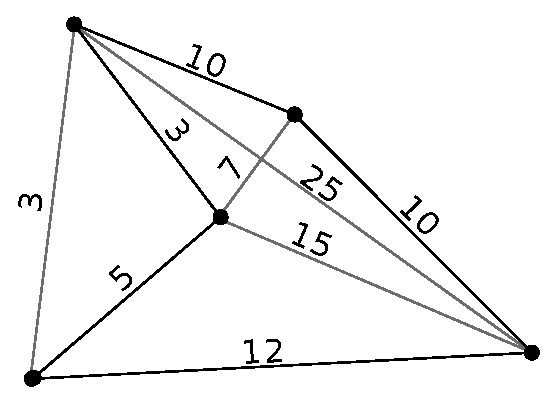
\includegraphics[height=3cm]{complexity/langcomplexity/pictures/tsp}
\end{center}
\begin{example}[Relevance]
	A circuit is basically a round-trip over a board. As such, minimizing 
	the resistance, \dots encompasses solving the TSP.
\end{example}

\paragraph{Satisfiability of boolean expressions (SAT)}
Given a boolean expression with variables, is there a way to assign the 
variables, so that the whole expression is true?
\begin{example}[Relevance]
	When modelling certain domains, for example in a system of artificial
	intelligence, constraints are often expressed as boolean expressions or can
	be converted to them\footnote{See \cite{russell1995artificial}}. Checking
	whether the constraints can be satisfied at all can already solve problems:
	If we have the facts $F$ and the hypothesis $H$, then $H$ fits the facts, if
	and only if $F\wedge\lnot H$ is \emph{not} satisfiable.
\end{example}
\subsubsection{Polynomial reductions}
SAT is an extremely handy problem to reduce to, so the following reductions 
will mostly feature that.
\paragraph{SAT reduces to TSP}
It can be shown, that SAT can be reduced to a special case of itself, namely 
$3-cnf SAT$, the satisfiability of formulas in the so-called 3-clause normal form

\[ \bigwedge_{i=1}^n a^1_i\vee a^2_i \vee a^3_i \].
where $a^j_i$ can be any $x_k$ or $\lnot x_k$. The 
$a^1_i\vee a^2_i \vee a^3_i$ are known as the \emph{clauses}.

How this could be done might become apparent when looking at the proof of
theorem~\ref{sat-np}. Without loss of generality then, we can assume, that 
the formula is in this form, when we try to reduce it to TSP. This has the 
advantage, that we know, that all clauses must be true and that in all 
clauses, one of the atoms must be true.

TSP takes as an input the maximum summed cost, but it is clear, that there is 
a special case, in which only the existance of a round-trip is asked for, not 
the limit of the cost\footnote{One could for example set all costs to zero 
and check for any number $M$}. This case is known as the Hamiltonian Cycle problem.

Now we need to create a graph, that is polynomially large in the length of 
the formula, but contains a round-trip if and only if the formula is 
satisfiable. The trick is of course using the clause-normal-form: Represent 
all clauses as a node $n_k$. The idea is now to only allow connections to 
$n_k$, if the representation of the atom makes the clause true\footnote{This 
construction is based on \cite[p. 286-291]{sipser2006introduction}}.

Variables have a more complex structure

\begin{itemize}
	\item a start node, in which the decision takes place, if the variable is 
		set to $True$ (left) or $False$ (right). Depending on choice, the steps 
		through the middle will allow of disallow checking off clauses.
	\item a bridge in the middle, that can either be just walked through, but 
		also has some connections to the $n_k$ nodes that will be explained shortly.
	\item an end node, which will be the start node to the next variable.
\end{itemize}

\begin{figure}[htb]
	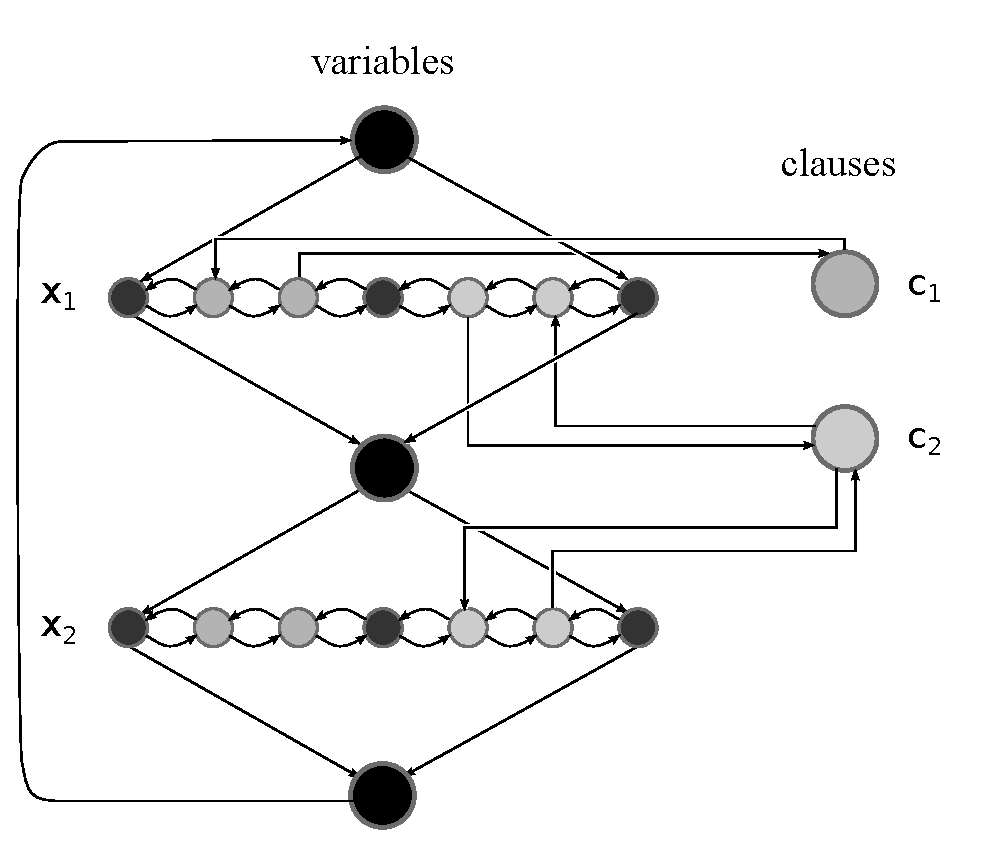
\includegraphics[width=0.97\textwidth]{complexity/langcomplexity/pictures/satastsp}
	\caption{The tour for the expression $(x_1\vee\lnot x_2)\wedge x_2$}
	
\end{figure}

It is clear, that the only 
round-trip possible leads through assigning all variables true or false, but 
we don't have a coding for \emph{variable $i$ appears in clause $j$}. 

This is done with giving meaning to the hops on the bridge: If the variable 
$i$ makes $j$ true if taken as $True$, then the $j$th such pair contains 
a hop from the left node to the right one over $n_j$, and from the right to 
the left, if assigning $False$ makes $j$ true.

\begin{theorem}
	This construction has a round-trip if and only if the original formula is satisfiable.
\end{theorem}
\begin{proof}
	If the formula is satisfiable, then we can tick off one clause after 
	another, by taking the hops from the bridge to $n_k$ whenever possible. 

	Now if the formula is \emph{not} satisfiable, then that means, that at 
	least one clause cannot be made true, but that translates directly to not 
	bein able to jump over to it with the current variable assignment in the graph.
\end{proof}
\paragraph{TSP reduces to SAT}
Lets reduce the TSP for the graph $G = (Nodes, Edges)$ for at most the cost
$M$ to a problem of satisfiability of boolean expressions.

We first notice, that we can add and compare numbers by building a fixed 
length binary calculator from the logical connectives, that is able to add 
all weights if necessary. This won't require to introduce more than 
polynomial many variables and connectives.

Let the variables $p_i^n$ denote, that the $i$th node of the path is $n$, 
then 
\[ PathExclusion = \bigwedge_{i=1}^{\abs{Nodes}}\bigwedge_{n\in Nodes} \bigwedge_{n'\in Nodes\atop n'\neq n} p_i^n \rightarrow \lnot p_i^{n'}\]
says that at any given position, only one node can be visited. Now we can 
just add up all weights multiplied with $1$ if they are in the round-trip or 
$0$ if they are not. This would look messy, because we have to do it bitwise, 
but the solution would look like
\[
	PathExclusion \wedge \left( \sum_{e=\in Edges} cost(e)\cdot 
	include\mhyphen edge(e) \right) \]
where 
\[ include\mhyphen edge(n_0, n_1)= \begin{cases}
		1, &\text{if }\bigvee_{k=1}^{\abs{Edges}} p_k^{n_0} \wedge p_{k+1}^{n_1}\\
		0, &\text{otherwise }
	\end{cases}\]

This formula would still be polynomially long in the input length and 
wouldn't contain any predicates. Therefore, it is polynomially reduced 
to $SAT$.
\DONE
\paragraph{Factorization reduces to TSP}
Factorization would be very easy to reduce to SAT: Given a $n$ digit binary 
number $z$, we could device $a_i$ and $b_i$ for $i=1\ldots (n-1)$ as $n-1$ digit 
binary numbers. We could then build a binary multiplier\footnote{Consult your 
favourite book on computer engineering} and check, if the result is the same 
as $z$. But we already found, that any SAT problem can be reduced to TSP, so 
if we use the construction with the zick-zack-gates again and on a large 
scale, we can convert $a_i$ and $b_i$ and the binary multiplier. Since 
applying two polynomial reductions in series still is a polynomial reduction, 
we can reduce Factorization to TSP. 
% Not sure, if I should do a smarter way, but then again, maybe there is no 
% elegant way...

\paragraph{CFG reduces to SAT}
Here as well, it is useful to use a special form, in order to manage the 
complexity that the problem in unrestricted form offers: Context-free 
grammars can (relatively easily with a mere $n^4$ blow up of the grammar) be
converted to the so called Greibach Normal Form, in which rules always have one
of the following forms:

\begin{align*}
	X &\rightarrow \alpha, A_1, A_2, \ldots, A_n \\
	S &\rightarrow \varepsilon
\end{align*}

where $A_i$ are non-terminals and $\alpha$ is a terminal. Furthermore $\varepsilon$ 
denotes the empty string and $S$ the start symbol.

This form has some consequences, for example that only one rule if any can 
produce empty strings, all others produce at least one terminal. Another nice 
property is that the string grows to the right, we don't \emph{need} to go 
back if we perfer not to.

In this case, we will just expand the left-most non-terminal one after 
another until the string is fully produced -- after at most $n$ steps, since 
we don't need to use the empty string rule, except when explicitly matching 
the empty string. Now let $R_t^r$ denote that we use the rule $r$ at the step $t$.
Since we expand one after another, we need to formalize exclusion as seen earlier:

\[ RuleExclusion = \bigwedge_{t=1}^{n}\bigwedge_{r\in Rules} \bigwedge_{r'\in Rules\atop r'\neq r} R_t^r \rightarrow \lnot R_t^{r'}\]

Furthermore we need to model the string after the step $t$, by defining 
$S^A_{x,t}$ to mean that the $x$th symbol of the string is $A$ at the time $t$. 
Again, we exclude the possibility, that the string has multiple symbols at 
the same time and space.

\[ SymbolExclusion = \bigwedge_{t=1}^{n}\bigwedge_{x=1}^{n}\bigwedge_{s\in Symbols} \bigwedge_{s'\in Symbols\atop s'\neq s} S_{x,t}^s \rightarrow \lnot R_{x,t}^{s'}\]

With these at our disposal, we can define the expansion rules: 
$Rule_j = X \rightarrow \alpha, A_1, \ldots, A_m$ becomes 
$\coded{Rule_j} = S^X_{i,t}\rightarrow S^\alpha_{i,t+1}\wedge \bigwedge_{k=1}^m S^{A_k}_{i+k, t+1}$

Then the matching of context-free grammars can be solved by solving

\[ RuleExclusion \wedge SymbolExclusion \wedge \bigwedge_{t=1}^{n}\bigvee_{j = 0}^{\abs{Rules}} \coded{Rule_j} \]

\subsection{Hardness and completeness}
We saw that in computability, there seems to be a natural border of 
computability, in which \WHILE, Turing machines and nearly any reasonably 
strong language reside. It was not too surprising then, that these different 
languages could express each other and themselves by means of interpretation and
compilation. Maybe more surprising is, that the complexity classes \PTIME and 
\NPTIME seem to be a similarly natural border.

\begin{defn}
	For a complexity class $C$, a problem $P$ is \emph{hard}, if 
	$\forall c\in C: c \reducesTo_{\PTIME} P$.

	The problem $P$ is \emph{$C$-complete}, if $P$ is $C$-hard and $P\in C$.
\end{defn}
\begin{example}
	\begin{itemize}
		\item \FOR is \PTIME-hard, but not complete, because not all \FOR programms run in \PTIME.
		\item \TM is \WHILE-complete.
	\end{itemize}
\end{example}
These examples are a bit cheated, since they use extremely large complexity 
classes. But in fact, we have seen two problems already, that are \NPTIME-complete.

\subsubsection{SAT is \NPTIME-complete}
\begin{theorem}
	\label{sat-np}
	The satisfiability of boolean formulas is \NPTIME-complete.
\end{theorem}
\begin{proof}
	For completeness, inclusion and universality are required.

	To prove $SAT\in \NPTIME$, we use the guess-and-check definition of 
	\NPTIME. The required certificate in this case is a mapping of the variables to 
	truth-values. This is at most linear in the length of the expression, 
	therefore fulfilling the required \PSPACE length of the certificate. Given the 
	certificate, we can then fully evaluate the expression, which again takes 
	linear time.

	The general idea how to create an $X$-complete problem is to simulate the 
	mode of computation. In the case of space completeness, you fail if you 
	move out of a premarked part of the tape, in the case of 
	\PTIME-completeness, you count down your remaining time and in the case of 
	\NPTIME-completeness, you build a table of possible configurations of the 
	turing machine and see if any of them succeeds\footnote{This proof combines 
		ideas from the proofs given by \cite{jones} and \cite{sipser2006introduction}}.

	% Jones has a more elegant approach, but that requires to introduce the 
	% language SBoole, which then simulates a GOTO program, which simulates a 
	% TM. However the solution is so much prettier, that I consider adapting it 
	% to the known formalisms.
  %
	First of all, it is not necessary to use transition function 
	$\delta: Q\times \Gamma \rightarrow \mathcal{P}(Q\times \Gamma\times \{L, N, R\})$
	, it is sufficient to be able to choose between two alternatives. If for 
	example $\delta(q, x) = \set{(q_1, y_1, d_1), \ldots, (q_n, y_n, d_n)}$, 
	then we can simply and polynomially reduce it to a list of binary 
	choices\footnote{The use of tuples instead of sets stems from the fact, 
	that one cannot speak of the \emph{first} or \emph{second} element of a 
	set, but for strict semantics, this is necessary.}:
	\begin{align}
		\delta(q, x) &= \Big((q_1, y_1, d_1), (q^{(1)}, x, N) \Big)\\
		\delta(q^{(1)}, x) &= \Big((q_2, y_2, d_2), (q^{(2)}, x, N) \Big)\\
		&\vdots \\
		\delta(q^{(n-1)}, x) &= \Big((q_{n-1}, y_{n-1}, d_{n-1}), (q_{n}, y_{n}, d_{n}) \Big)
	\end{align}
	So without loss of generality, we can assume, that the non-deterministic 
	Turing machine makes at most binary choices, which we could code as 
	booleans. Further, if we \emph{don't} want to make a choice, we could make 
	a choice, but end in $q_{reject}$ as the second option, so we can make 
	\emph{exactly} one binary choice per step.

	So let us now reduce the arbitrary problem $A\in\NPTIME$ to $SAT$. Since it 
	is polynomial runtime, there is some $k$ for which the runtime is bound by 
	$p(n) = n^k$.

	Even assuming, that we made a choice in every step, it would be enough to
	give $p(n)$ booleans $c_1, \dots, c_{p(n)}$ to fully specify the trace. This
	will be, what the solver for SAT would then modify to find the solution to
	$A$, the rest is deterministic. 

	The coding, if a trace ends in an accepting state, remains to be done -- 
	which includes coding how a Turing machine works. 

	The state changes over time, and has $\abs{Q}$ exclusive possibilities.
	Then $s^q_{t}$ means, that the machine is in state $q$ at the time $t$. 
	Coding, that the possibilities exclude each other can be done by adding 
	\begin{align}
		StateExclude &= \bigwedge_{q\in Q \atop t=1\ldots p(n)}{
		\bigwedge_{q'\in Q\atop q' \neq q}{s^q_{t} \rightarrow \lnot 
		s^{q'}_{t} }}\\
		&= \bigwedge_{q\in Q \atop t=1\ldots p(n)} 
		\bigwedge_{q'\in Q\atop q' \neq q} \lnot s^q_{t} \vee \lnot 
		s^{q'}_{t}
	\end{align}
	This gives $\abs{Q}^2\,p(n)$ additional input characters -- nothing that would 
	break polynomial input to $SAT$.

	The tape only needs $p(n)$ cells, but for each of the $p(n)$ time steps, 
	therefore we code the tape as the table $T^c_{x, t}$ with $c\in\Gamma$, 
	$x = 1\ldots p(n)$ and $t=1\ldots p(n)$, meaning \emph{the tape cell $x$ 
	contains the character $c$ at the time $t$}. The constraint is of course, 
	that at any given time, the tape at a given cell can only contain one 
	character, but this can be expressed by
	\begin{align}
		TapeExclude &= \bigwedge_{g\in \Gamma}\bigwedge_{x=1\ldots p(n) \atop t=1\ldots p(n)}
		\bigwedge_{g'\in \Gamma\atop g' \neq g}{T^g_{x,t} \rightarrow \lnot 
		T^{g'}_{x,t} }\\
		&= \bigwedge_{g\in \Gamma}\bigwedge_{x=1\ldots p(n) \atop t=1\ldots p(n)} 
		\bigwedge_{g'\in \Gamma\atop g' \neq g} \lnot T^g_{x,t} \vee \lnot 
		T^{g'}_{x,t}
	\end{align}.
	Despite looking huge at first glance, this is still polynomially long in the input.

	We also need to keep track of where the read/write head of the Turing 
	machine is. Perhaps unsurprisingly, we introduce a table $H_{x,t}$, meaning 
	that at the time $t=1\ldots p(n)$ the head is at the position 
	$x=1\ldots p(n)$. Exclusion applies, so we add
	\begin{align}
		HeadExclude &= \bigwedge_{x=1\ldots p(n) \atop t=1\ldots p(n)}
		{H_{x,t} \rightarrow \lnot H_{x,t} }\\
		&= \bigwedge_{x=1\ldots p(n) \atop t=1\ldots p(n)} \lnot H_{x,t} \vee \lnot 
		H_{x,t}
	\end{align}.

	Finally we need to code how the transitions take place. We need to say that
	\begin{itemize}
		\item Deterministically changing state means, that if we were in state $g$ 
			to time $t$ and saw the cell $T_x$ with the character $c$, then in $t+1$,
			we are in the state $g'$ implied by $\delta$.
			\begin{align}
				StateTransition^{q'}(s^q_t, T^c_{x,t}) 
									&= s^q_{t}\wedge T^c_{x,t} \rightarrow s^{q'}_{t+1}\\
									&= \lnot s^q_{t} \vee \lnot T^c_{x,t}\vee s^{q'}_{t+1}
			\end{align} 
		\item Deterministically changing the current cell does the same thing, 
			only with cells instead of states.
			\begin{align}
				CellTransition^{c'}(s^q_t, T^c_{x,t}) 
									&= s^q_{t}\wedge T^c_{x,t} \rightarrow T^{c'}_{x,t+1}\\
									&= \lnot s^q_{t} \vee \lnot T^c_{x,t}\vee T^{c'}_{x,t+1}
			\end{align} 

		\item Deterministically moving on the tape only changes $H_{t+1}$
			\begin{align}
				MoveTransition^d(s^q_t, T^c_{x,t}) 
				&= s^q_{t}\wedge T^c_{x,t} \wedge H_{x,t} \rightarrow H_{x+d,t+1}\\
									&= \lnot s^q_{t} \vee \lnot T^c_{x,t}\vee H_{x,t}\vee H_{x+d,t+1}
			\end{align},
			where $d\in \set{-1,0,1}$
		\item If our current choice bit says $True$, then take the first option $X_t$, 
			else the second option $Y_t$. This could for example be expressed by 
			$(c_t \wedge X_t) \vee (\lnot c_t \wedge Y_t)$.

		\item Plugging this together, we get the coding of the transition 
			function.
			\begin{multline}
				FirstTransition_{x,t} 
				= H_{x,t}\wedge T^c_{x,t}\wedge s^q_{t} \rightarrow
				\\ MoveTransition^{d}(s^q_t, T^c_{x,t}) \wedge 
				\\ CellTransition^{c'}(s^q_t, T^c_{x,t}) \wedge
				\\ StateTransition^{q'}(s^q_t, T^c_{x,t}) \\
			\end{multline}
			if $\delta(c,q) = \left((c', q', d), (c'', q'', d')\right)$ and analogously for 
			the second choice
			\begin{equation}
				Transition = \bigwedge_{t=1}^{p(n)}\bigwedge_{x=1}^{p(n)} 
							(c_t \wedge FirstTransition_{x,t}) \vee 
							(\lnot  c_t \wedge SecondTransition_{x, t})
			\end{equation}

			Even this huge transition table is still polynomial in the length of the input.
	\end{itemize}
	
	Finally, the formula should only be accepted of the end state is $q_{accept}$, which is simply $EndState = s^{q_{accept}}_{p(x)}$.

	Now $Transition\wedge HeadExclude \wedge TapeExclude \wedge StateExclude \wedge EndState$ 
	is the representation of $A$ in $SAT$. Note that no functions (predicates) would have 
	been necessary\footnote{Slightly changing this proof shows then, that predicate 
	logic is actually Turing complete.}.

	With this so-called \emph{gadget} -- something that simulates the 
	computational behaviour of another problem -- we have reduced the problem $A$ 
	to $SAT$. Basically we reduced the problem of calculating $p(n)$ steps on a 
	non-deterministic Turing machine, which is by definition \NPTIME-complete, 
	to the $SAT$ problem.
\end{proof}
This implies, that SAT can express any other \NPTIME problem with only a 
polynomial slowdown. This also means, that SAT could model any \PTIME 
problem, such as checking context free grammar membership.

On the other hand, we saw that SAT can be reduced to the Traveling Salesman 
Problem, which shows its completeness as well.

There are indeed many relevant problems that are \NPTIME-complete\footnote{So 
many in fact, that the author struggled to find any interesting \PTIME-complete
problems}, for example maximizing linear functions over linear constraints in
the domain of integers or optimal scheduling of tasks over multiple processors
just to name two.

\subsubsection{\NPTIME and optimization}
\label{np-opti}
While one should keep in mind, that \NPTIME only
describes decision problems, many \NPTIME-complete
problems actually hide an optimization problem. For
example, if we can determine if the traveling
salesman can do the round-trip with cost of at most
$k$, then we can actually find the optimal path:

\begin{algorithmic}[1]
	\State find least $k_0$, so that the round-trip is possible with binary search over $k$
	\For{each edge $e$ in the graph}
		\State Remove $e$ from the graph
		\State Check if the round-trip cost increases
		\State If so, reinsert $e$
	\EndFor
\end{algorithmic}

After the algorithm finishes, the only edges in the graph are the ones in the round-trip.

Why does this work? First the binary search determines the exact cost of the optimal route and does so in only $\log k_0 \cdot f(x)$, where $f(x)$ is the time that TSP takes. 

The loop then uses that any edge, that is not in the round-trip will leave the cost untouched, even when removed. An edge, that can not be compensated however will increase the cost, when removed. If there are more than one possible round-trip with the same cost, then only one of them will survive the loop, because edges will be removed, if any of the routes is still possible. We would need $\abs{E}\cdot f(x)$ time for the loop.

All in all this algorithm will take $(\log k_0 + \abs{E})\cdot f(x)$ and therefore has only a linear slowdown compared to solving TSP.

\subsubsection{Help, my problem is \NPTIME-complete}
While being (probably) asymptotically very difficult to solve, 
\NPTIME-complete problems are by no means impossible. There are some 
strategies that can be applied to handle them.
\paragraph{\NPTIME-complete does not necessarily mean slow}
In many cases, the precise algorithm to solve the problem works reasonably 
fast in most cases, but explodes for some abnormal cases. If these abnormal 
cases don't occur in normal input data, the algorithm is still save.

For example, if we are solving SAT, but the inputs take only the form of horn 
clauses (for example $\bigwedge x_i \rightarrow y$), then the problem is 
solvable in \PTIME. 

It could also be, that the algorithm runs in $\mathcal{O}((1+\varepsilon)^n)$ 
for some small $\varepsilon$. Then $n$ would have to be very big for it to be problematic.
\paragraph{Parametrization}
The problem might be slow in general, but there are different parameters to 
the problem, that, when fixed, make the algorithm polynomial. Only increasing 
these parameters then give the full problem. 

For example, checking if a given program in the ML language\footnote{Java or
	C++ would be no better as anyone who ever used template code knows. Actually,
	C++ templates are even Turing-complete \cite{veldhuizen2003c++}}
does not violate any typing (i.e.\ a cast would be necessary) is
\NPTIME-complete\footnote{See \cite{downey1999parameterized}}, but if we
parametrize by the number of type definitions in the system, we have merely a
polynomial runtime.
\paragraph{Approximation}
As seen in section~\ref{np-opti}, many \NPTIME-complete problems are actually
optimization problems in disguise. Instead of looking for \emph{the} optimal
solution, often it is enough to settle for a sub-optimal, but good enough
solution.  In this text, we didn't develop the necessary tools to analyse such
inaccurate algorithms, but such algorithms can come --provably-- very close to
an optimal solution, while taking only polynomial time.

\subsection{Other complexity classes}
The complexity classes introduced are of course only scratching the surface 
of the fascinating topic of complexity theory. There are many different modes 
of computation, that do not factor into \PTIME or \NPTIME, for example 
parallelism, which will be of ever greater importance, as the number of cores 
of computers increase, when the sequencial speed cannot. A bit further down 
the road, the quantum computer will get its share.

\paragraph{$\mathtt{NC}$}
stands for Nick's class\footnote{honoring Nick Pippenger} and
has been described as the class of well-parallelizable 
problems\footnote{See \cite{sipser2006introduction}}. It is known that $\mathtt{NC} \subset \PTIME$, but it is unknown, 
whether this inclusion is proper. Similarly to \NPTIME-complete problems, 
\PTIME-complete problems, such as CFG, are analyzed to prove this. 

\paragraph{$\mathtt{BQP}$}
is the class of bounded-error polynomial-time quantum computable decision 
problems. Bounded error compensates for the fact that quantum computation is, 
in order to achieve its full strength, random. Bounding the error means that 
it gives the wrong answer at most $0<\varepsilon<\frac{1}{2}$ of the time, where 
$\varepsilon$ is often arbitrarily chosen to be $\frac{1}{3}$. Given a 
procedure in $\mathtt{BQP}$, it is easy to see, that we can lower the 
probability of error arbitrarily low by running the procedure multiple times 
and taking the average answer.

It is possible to simulate a quantum computation in \PSPACE, and it is 
possible to simulate a deterministic computation on a quantum computer, so 
$\PTIME \subset \mathtt{BQP} \subset \PSPACE$, but again, all inclusions are 
suspected, but not proven, to be proper.

The connection to \NPTIME is unknown, but $\NPTIME\subset \mathtt{BQP}$ would 
imply $\NPTIME\neq \PTIME$.